\section{Methods and Materials}
\label{sec:methods}



% Talk about what you plan to do in the Fall. 
% Describe so that they can be replicated. 

In the fall, I plan to use the RoboRoach kit (Backyard Brains; Ann Arbor, MI) kit to apply electrical stimulation to a cockroach's antenna, causing it to turn in the contralateral direction when I apply current. The kit includes a printed circuit board (PCB), which is a backpack that carriers the Bluetooth Low Energy wireless receiver/transmitter, which will allow communication between my smartphone and the backpack. It includes a battery for the backpack and three electrode sets for three cockroaches, each of which include one electrode for each antenna and one for ground, since electricity needs a closed circuit and the electrical stimulation current needs a return pathway. The kit also consists of all the items necessary for surgery: fine forceps (tweezers), forceps (hemostat), a loupe, a low temperature hot glue gun, hot glue sticks, Q-tips, sandpaper, loctite super glue, a popsicle stick, silly putty, dissection scissors, flour, a needle, and toothpicks. In addition to the kit, I will need a cup of ice water, paper towels, a clock, and a work lamp. I will use the Backyard Brains instructions to implement the surgery on the cockroaches.




\subsection{Experimental subjects}
I will order two species of cockroaches to evaluate a possible difference in performance based on species. I will order at least five adult \emph{Periplaneta americana} (American cockroaches) and three adult \emph{Gromphadorhina portentosa} (Madagascar hissing cockroaches). I will keep them in separate terrariums, with plenty of food, water, and space to move around.






\subsection{Surgery}
The surgery alone should only take \SIrange{30}{45}{\minute} , but I will allot \SI{1}{\hour} for the entire experiment considering set up and clean up time. I will conduct surgery on the cockroaches one at a time. After preparing my work station, I will anesthetize the cockroach by submerging it in the ice water until it falls asleep. 

% All the sub-bits here would normally go in the appendix.
\subsubsection{Attach the electrode array}
Once the roach is fully anesthetized, I will carefully place the cockroach on my table. Then I will grasp the pronotum, the exoskeleton ``hood'' over the head, and lightly sand the center of the pronotum until it feels slightly rough to the touch. 
{\begin{figure}[ht!]
\centering
\includegraphics[scale=0.25]{Surgery Photos/sand.jpg}
\caption{Sand the pronotum}
\label{fig:sand}
\end{figure}}
After, I will wipe the pronotum with a wet towel and dry it completely with a paper towel. 
{\begin{figure}[ht!]
\centering
\includegraphics[scale=0.15]{Surgery Photos/wipe.jpg}
\caption{Wipe off the pronotum}
\label{fig:wipe}
\end{figure}}
I will put a dab of superglue on the sanded area. 
{\begin{figure}[ht!]
\centering
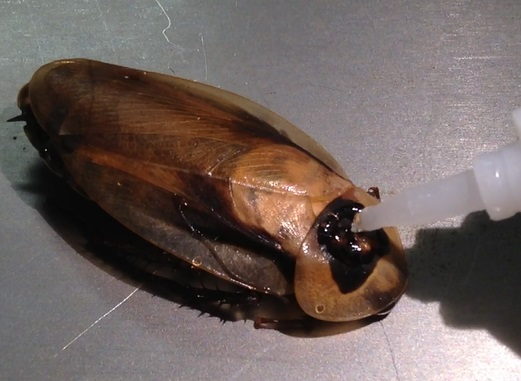
\includegraphics[scale=0.25]{Surgery Photos/gluepronotum.jpg}
\caption{Dab of glue on the pronotum}
\label{fig:gluepronotum}
\end{figure}}
With the electrodes facing towards the antennae, I will gently place the black connector on the glue so that the pins are parallel to the length of the body. 
% I CAN'T GET THIS FIGURE W 2 SUBFIGURES TO WORK??
\begin{figure}[ht!]
\centering
    \begin{subfigure}{.4\textwidth}
    \centering
    \includegraphics[scale=0.3]{Surgery Photos/connector1.JPG}
    \caption{Square black connector}
    \label{fig:connector1}
    \end{subfigure}
    \begin{subfigure}{.4\textwidth}
    \centering
    \includegraphics[scale=0.3]{Surgery Photos/connector2.JPG}
    \caption{Place connector on glue dab}
    \label{fig:connector2}
    \end{subfigure}
\caption{Placing the black connector}
\label{fig:connector}
\end{figure}
After the glue to bonds to the black connector, I will place the roach back into the ice water to ensure that it is still anesthetized.

\subsubsection{Implant the ground electrode}
I will place the roach on the table, belly down and splay its wing to the side, using silly putty to hold the wing down and stabilize it. 
{\begin{figure}[ht!]
\centering
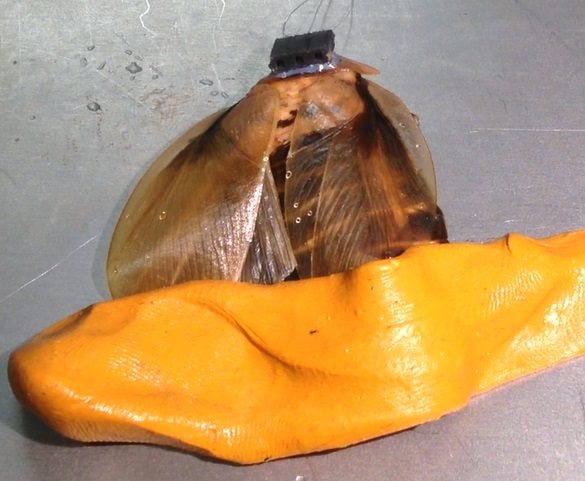
\includegraphics[scale=0.25]{Surgery Photos/putty.jpg}
\caption{Hold the wing down}
\label{fig:putty}
\end{figure}}
I will dry its thorax and then lightly sand it. Using the needle and avoiding the center line, I will lightly poke a small hole in the exoskeleton of the thorax, just behind its head. 
{\begin{figure}[ht!]
\centering
\includegraphics[scale=0.5]{Surgery Photos/avoidesoph.jpg}
\caption{Avoid the esophagus}
\label{fig:avoidesoph}
\end{figure}}
{\begin{figure}[ht!]
\centering
\includegraphics[scale=0.3]{Surgery Photos/hole.jpg}
\caption{Poke hole here}
\label{fig:hole}
\end{figure}}
With the tweezers I will insert the electrode 1mm into the hole I just made and then I will apply a small bead of super glue to the electrode.
{\begin{figure}[ht!]
\centering
\includegraphics[scale=0.4]{Surgery Photos/celectrode1.jpg}
\caption{Insert the center electrode}
\label{fig:celectrode1}
\end{figure}}
I will insert the electrode \SIrange{1}{3}{\milli\meter} into the hole, allowing the superglue to enter the body. 
{\begin{figure}[ht!]
\centering
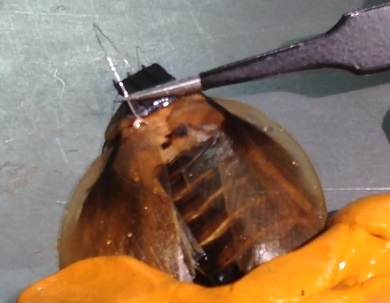
\includegraphics[scale=0.4]{Surgery Photos/celectrode2.jpg}
\caption{Insert the center electrode further}
\label{fig:celectrode2}
\end{figure}}
I will replace the right wing to its resting place and allow the glue to set. Once I believe it has set, I will lightly tug to test if the ground electrode is secure. Lastly, I will return the cockroach to the ice water for \SIrange{1}{2}{\minute} to maintain anesthetization.

\subsubsection{Implant the right antenna electrode}
I will take the roach out of the ice water and splay the antenna out. I will cut the cockroach's right antenna to \SIrange{3}{6}{\milli\meter}. 
{\begin{figure}[ht!]
\centering
\includegraphics[scale=0.3]{Surgery Photos/cut.jpg}
\caption{Cut the right antenna}
\label{fig:cut}
\end{figure}}
I will insert the right electrode 1 mm inside the right antenna, not all the way in. 
{\begin{figure}[ht!]
\centering
\includegraphics[scale=0.3]{Surgery Photos/relectrode1.jpg}
\caption{Insert the right electrode}
\label{fig:relectrode1}
\end{figure}}
Then I will dab a bead of super glue just above where the electrode is in the antenna. 
{\begin{figure}[ht!]
\centering
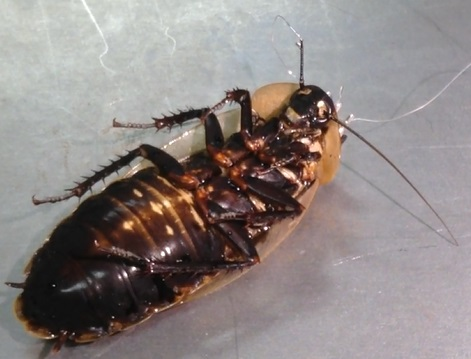
\includegraphics[scale=0.3]{Surgery Photos/relectrodeglue.jpg}
\caption{Apply a dab of glue}
\label{fig:relectrodeglue}
\end{figure}}
I will insert the electrode so that the bead of glue partially enters \SIrange{2}{4}{\milli\meter} into the antenna. The goal is to get the glue just inside the inner ring of the antenna so the electrode will not fall out easily. 
{\begin{figure}[ht!]
\centering
\includegraphics[scale=0.3]{Surgery Photos/relectrode2.jpg}
\caption{Insert the right electrode further}
\label{fig:relectrode2}
\end{figure}}
I will then put the roach back into the ice water for \SIrange{1}{2}{\minute} to maintain anesthetization.

\subsubsection{Implant the left antenna electrode}
\begin{figure}[ht!]
\centering
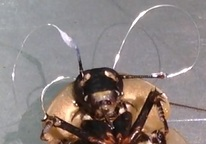
\includegraphics[scale=0.7]{Surgery Photos/lelectrode.jpg}
\caption{All electrodes in}
\label{fig:lelectrode}
\end{figure}
This section is the reverse of the previous. The cockroach should look like \fref{fig:lelectrode}.

\subsubsection{Tighten wire slack}
Because cockroach legs are strong and can pull the electrodes out if they get snagged, it is important to tighten the wire slack. I will fold back the wire slack on top of the connector, minimizing the amount of slack wire between the antenna and connector and not allowing the exposed parts of silver wire to touch. 

\begin{figure}[ht!]
\centering
    \begin{subfigure}{.49\textwidth}
    \centering
    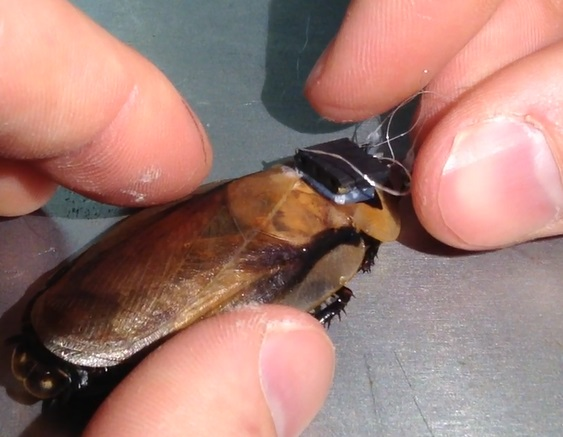
\includegraphics[scale=0.25]{Surgery Photos/nowire.JPG}
    \caption{Fold the wire slack}
    \label{fig:nowire}
    \end{subfigure}
    \begin{subfigure}{.49\textwidth}
    \centering
    \includegraphics[scale=0.4]{Surgery Photos/nowire2.JPG}
    \caption{Minimize wire slack}
    \label{fig:nowire2}
    \end{subfigure}
\caption{Tighten wire slack}
\label{fig:connectorB}
\end{figure}
I will wet and then dip the end of the popsicle stick in flour. In order to hold the excess wire in place, I will take the glue gun and place a dab of hot glue on the wires, quickly using the flour end of the popsicle stick to smush down the glue. 
\begin{figure}[ht!]
\centering
    \begin{subfigure}{.49\textwidth}
    \centering
    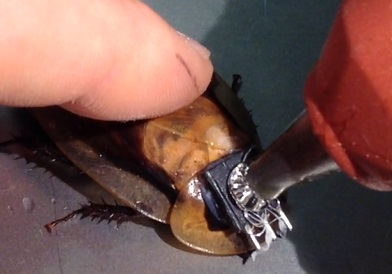
\includegraphics[scale=0.4]{Surgery Photos/gluewires.jpg}
    \caption{Apply a dab of hot glue}
    \label{fig:gluewires}
    \end{subfigure}
    \begin{subfigure}{.49\textwidth}
    \centering
    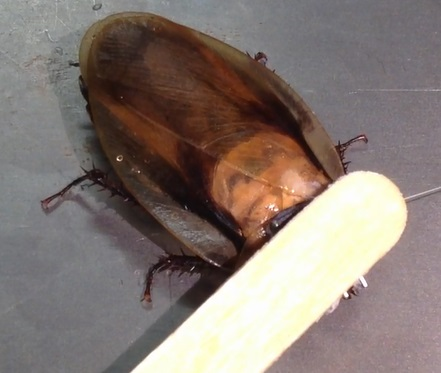
\includegraphics[scale=0.3]{Surgery Photos/gluewires1.jpg}
    \caption{Mash with the popsicle stick}
    \label{fig:gluewires1}
    \end{subfigure}
    \begin{subfigure}{.49\textwidth}
    \centering
    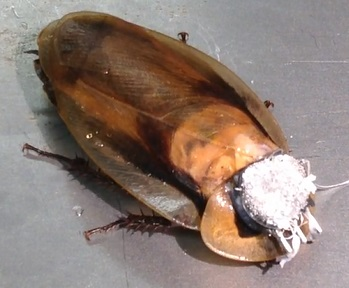
\includegraphics[scale=0.4]{Surgery Photos/gluewires2.jpg}
    \caption{Final product}
    \label{fig:gluewires2}
    \end{subfigure}
\caption{Glue the wires together}
\label{fig:connectorC}
\end{figure}

\subsubsection{End of surgery}
Once the surgery is complete, I will place the roach back in its terrarium, giving it at least \SIrange{2}{4}{\hour} if not a full night to recover. This surgery will be repeated for each cockroach participating in the experiment.







\subsection{Testing}
Before testing, I will download the RoboRoach app from the app store. To test my stimulation of the antennae, I will plug the male connector of the PCB into the female connector on the roach's head. I will press the small black button on the
left edge of the PCB to awaken the microcontroller. From my phone, I will use the default stimulation settings and swipe left or right to observe behavioral responses. The surgery is successful if the cockroach turns in the direction I swiped.

To evaluate performance, I will lay thin strips of electrical tape on the ground at angles in increments of \ang{30}, ranging from \ang{0} to \ang{360}. I will start by placing the cockroach at \ang{0}, and then measure the angle of turn upon stimulation. 






















